\subsection{Setup}
The general setup of the experiment consists of a rotating pendulum, equipped with a electromagnetic brake and a motor as shown in Fig. \ref{fig::setup}.
\begin{figure} [ht]
	\centering
	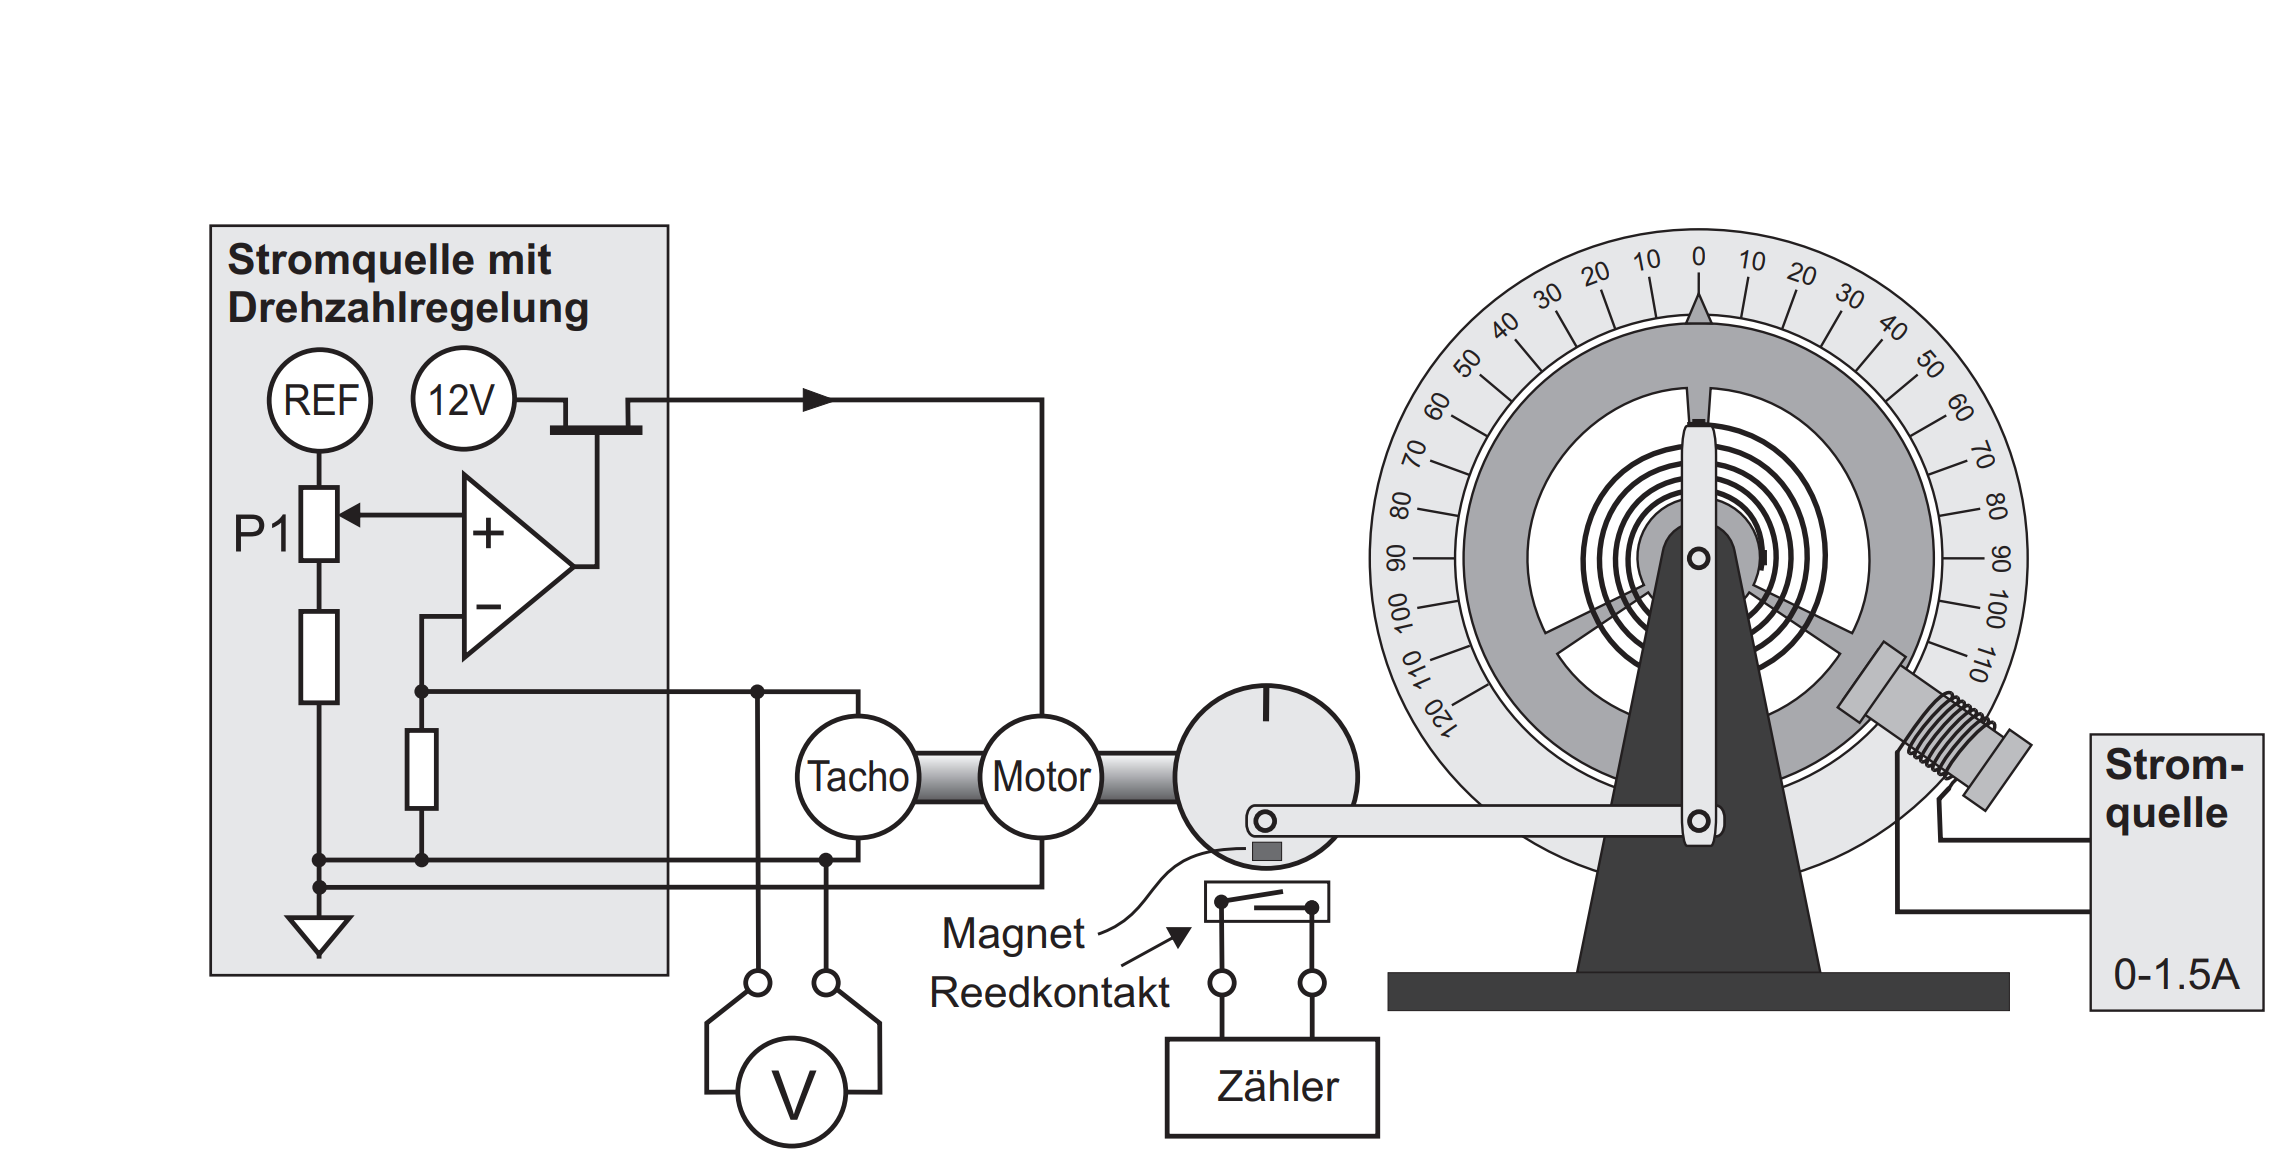
\includegraphics[width=400pt]{img/setup.PNG}
	\caption{Experiment Setup: Rotating pendulum with motor and electromagnetic brake. \cite{manual}}
	\label{fig::setup}
\end{figure}

The system itself would have some dampening caused by friction, but as we want to test different dampenings, we use the electromagnetic brake to create controlled dampening.
We want to determine the dampening constants $\alpha_{1, 2, 3}$ of the system for current values $I_{1, 2, 3}$ of the brake of 0.64, 0.9 and 1.2 A.